\section{Computed Tomography}

Computed Tomography (CT) is a non-invasive imaging technique that reconstructs the internal structure of an object from measurements taken externally. The term \textit{tomography} itself derives from the Greek words \textit{tomos} (slice or section) and \textit{graphein} (to write or record), which reflect its purpose of producing representations of a target by observing cross-sectional images of a target without physical intervention.

The physical principle underlying Computed Tomography relies on the transmission of waves or particles, most commonly X-rays, through the object of interest. As X-rays traverse matter, their intensity is attenuated according to the material's local properties. In the simplest homogeneous case, this relationship is captured by the exponential decay $I_1 = I_0 e^{-\mu s}$, where $I_0$ and $I_1$ denote the incident and transmitted intensities, $\mu > 0$ is the attenuation coefficient, and $s$ is the path length through the material. For non-homogeneous objects, this generalizes to $I_1 = I_0 \, e^{-\int_{\ell} \mu(x)\, dx}$. The \textit{Beer-Lambert law} can be used to connect the the initial and final intensities of an X-ray:

\begin{equation}
    I_1 = I_0 \, e^{-\int_{\ell} \mu(x)\, dx} \Longleftrightarrow -\log(I_1/I_0) = \int_{\ell} \mu(x)\, dx
\end{equation} 

As a result, during a tomographic scan, $I_0$ is known from calibration and $I_1$ from measurements. $I_1$ is measured along many lines $\ell_{(\omega,s)}$ to get many line integral values through the object. The intensity $I_1$ is called the \textit{transmission}, while the corresponding $-\log(I_1/I_0)$ is called absorption or \textit{projection}, and a collection of projections is called a \textit{sinogram}.

Mathematically, CT reconstruction can be cast as an inverse problem. Given a target $u \in X = L^2(\Omega)$ with $u \colon \mathbb{R}^d \to \mathbb{R}_+$ defined on a bounded domain $\Omega \subset \mathbb{R}^d$ ($d = 2, 3$), the \textit{forward problem} models the acquisition process via the Radon transform $\mathcal{R}(u) = y$, which integrates $u$ over lines $\ell(\omega, s)$ parameterized by $(\omega,s) \in S^1 \times \mathbb{R}$. The reconstruction task, i.e., recovering $u$ from measured data $y$, constitutes the corresponding \textit{inverse problem}.

The classical analytic solution to this inverse problem is \textit{Filtered Backprojection} (FBP), an exact inversion formula valid in the continuous setting. FBP performs well when complete projection data are available and the target can be assumed static. However, it suffers from theoretical limitations under discretization and provides no stability guarantees in realistic acquisition conditions.

In many practical scenarios, reducing the X-ray radiation dose or shortening scan time leads to \textit{limited data tomography}, which encompasses two main regimes: \textit{limited-angle CT}, where projections are acquired only within a restricted angular range, and \textit{sparse-angle CT}, where a reduced number of projection angles are sampled over the full range. Both settings cause FBP to produce severely degraded reconstructions, motivating the development of more advanced reconstruction methods capable of handling incomplete and noisy measurement data. Both scenarios can be seen in figure \ref{fig:fbprobe}.

\begin{figure}[h]
    \centering
    \begin{minipage}{0.8\linewidth}
        \centering
        \begin{subfigure}{0.49\textwidth}
            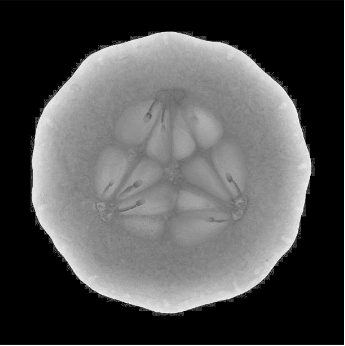
\includegraphics[width=\linewidth]{images/ctground.png}
            \caption{Ground truth}
        \end{subfigure}
        \hfill
        \begin{subfigure}{0.49\textwidth}
            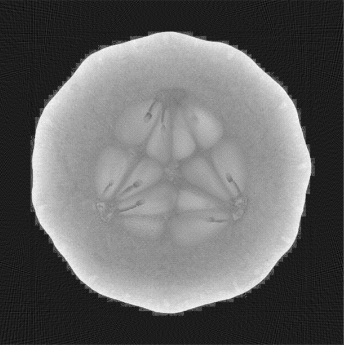
\includegraphics[width=\linewidth]{images/ctfullangle.png}
            \caption{FBP from full angle data}
        \end{subfigure}

        \vspace{0.5em}

        \begin{subfigure}{0.49\textwidth}
            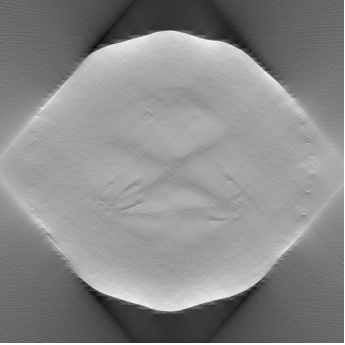
\includegraphics[width=\linewidth]{images/ctlimitedangle.png}
            \caption{FBP from limited-angle data}
        \end{subfigure}
        \hfill
        \begin{subfigure}{0.49\textwidth}
            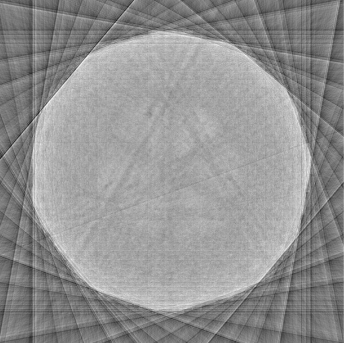
\includegraphics[width=\linewidth]{images/ctsparseangle.png}
            \caption{FBP from sparse angle data}
        \end{subfigure}

        \caption{Limited data tomography: examples.}
        \label{fig:fbprobe}
    \end{minipage}
\end{figure}